%**********************************************************************%
% _                    _                       _       _
% | |__   ___ _ __ ___ | |_ ___ _ __ ___  _ __ | | __ _| |_ ___
% | '_ \ / _ \ '_ ` _ \| __/ _ \ '_ ` _ \| '_ \| |/ _` | __/ _ \
% | |_) |  __/ | | | | | ||  __/ | | | | | |_) | | (_| | ||  __/
% |_.__/ \___|_| |_| |_|\__\___|_| |_| |_| .__/|_|\__,_|\__\___|
%                                        |_|
%----------------------------------------------------------------------%
\RequirePackage{plautopatch} %日本語パッケージを使う.
\documentclass[aspectratio=169, 12pt]{beamer} %  8pt, 9pt, 10pt, 11pt, 12pt, 14pt, 17pt, 20pt
\usetheme{Madrid}% テーマは指定しなくともよい.
%**********************************************************************%
% フォント
%----------------------------------------------------------------------%
\usepackage{luatexja} %日本語文書の組版を行う
\usepackage[T1]{fontenc} %アクセント記号をUTF-8で使用する.
\usepackage{inconsolata-nerd-font} %等幅フォント consolas
% 和文の既定フォントをゴシックに変更
\renewcommand{\kanjifamilydefault}{\gtdefault}
% Beamerによる数式フォントの置き換えを阻止
\usefonttheme{professionalfonts} 
%**********************************************************************%
% 数
%----------------------------------------------------------------------%
\usepackage{amsmath, amssymb} % 数式パッケージ
\usepackage{mathtools}
\usepackage{mathrsfs} %筆記体 $\mathscr{H}$ $\mathscr{L}$
\usepackage{bm} % for vector
%**********************************************************************%
% 図表
%----------------------------------------------------------------------%
\usepackage{here} %[H]オプション : 図表を文中のその場所に配置
\usepackage{ulem} % for \sout{} 取り消し線
\usepackage{booktabs} % \toprule \midrule \bottomrule
\usepackage{xcolor} %色
\usepackage{comment} %\begin{comment} \end{comment}でコメントアウト
\usepackage{boites} %ボックス内で改ページ可 
\usepackage{here, amsmath, latexsym, amssymb, bm, ascmac, mathtools, multicol, tcolorbox, subfig}

%**********************************************************************%
%      _                                       _
%   __| | ___   ___ _   _ _ __ ___   ___ _ __ | |_
%  / _` |/ _ \ / __| | | | '_ ` _ \ / _ \ '_ \| __|
% | (_| | (_) | (__| |_| | | | | | |  __/ | | | |_
%  \__,_|\___/ \___|\__,_|_| |_| |_|\___|_| |_|\__|
%**********************************************************************%



\begin{document}
%---------------------------------------------------------------
% タイトルスライド
%! 聞き流し数学2
\title{聞き流し数学I\hspace{-1.2pt}I}
\author[物理の計算屋]{物理の計算屋}
\date{}
\frame{\maketitle} % タイトルページ
%---------------------------------------------------------------
\begin{frame}{二項定理}
    %! 二項定理, aプラスbのn乗イコールシグマiイコール0からn, nCiaのnマイナスi乗bのi乗
    \begin{eqnarray*}
        (a+b)^n=\sum_{i=0}^n {}_nC_i a^{n-i}b^i
    \end{eqnarray*}
\end{frame}
%---------------------------------------------------------------
\begin{frame}{多項定理}
    %! 多項定理, aプラスbプラスcのn乗の一般項はp階乗q階乗r階乗分のn階乗aのp乗bのq乗cのr乗, ただし qプラスqプラスrイコールn, p, q, rは0以上, aプラスbプラスcのn乗の項数は3n, aのp乗bのq乗cのr乗の約数の数は括弧pプラス1括弧qプラス1括弧rプラス1
    \begin{center}
        $(a+b+c)^n$の一般項は$\frac{n!}{p!q!r!}a^pb^qc^r$ \par
        但し, $p+q+r=n$,\space$p\geq0, q\geq0, r\geq0$
    \end{center}
    \begin{center}
        $(a+b+c)^n$の項数$3n$ \par
        $a^pb^qc^r$の約数の数 $(p+1)(q+1)(r+1)$
    \end{center}
\end{frame}
%---------------------------------------------------------------
\begin{frame}{整数式の割り算}
    %! 整数式の割り算, A割るBの商q, 余りrとすると, AイコールBQプラスR (Rの次数ショウナリBの次数かRイコール0)
    \begin{center}
        $A \div B$の商$Q$, 余り$R$とすると, \par
        $A=BQ+R$\space ($R$の次数\space$<B$の次数\space か\space$R=0$)
    \end{center}
\end{frame}
%---------------------------------------------------------------
\begin{frame}{分数式}
    %! 分数式 B分のA掛けるD分のCイコールBD分のAC, B分のA割るC分のDイコール, B分のA掛けるC分のD, BC分のAD, C分のAプラスC分のBイコール, C分のAプラスB, C分のAマイナスC分のBイコールC分のAマイナスB
    \begin{eqnarray*}
        \frac{A}{B}\times\frac{C}{D} &=& \frac{AC}{BD} \\
        \frac{A}{B}\div \frac{C}{D}&=&\frac{A}{B}\times \frac{D}{C}=\frac{AD}{BC} \\
        \frac{A}{C}+ \frac{B}{C}&=&\frac{A+B}{C} \\
        \frac{A}{C}-\frac{B}{C}&=&\frac{A-B}{C}
    \end{eqnarray*}
\end{frame}
%---------------------------------------------------------------
\begin{frame}{恒等式の性質}
    %! 恒等式の性質, ax2乗プラスbxプラスcイコールaプライムx2乗プラスbプライムxプラスcプライムがxの恒等式, 同値, aイコールaプライム, bイコールbプライム, cイコールcプライム
    \begin{center}
        $ax^2+bx+c=a'x^2+b'x+c$が$x$の恒等式\par
        $\Leftrightarrow$ \space $a=a'$, $b=b'$, $c=c'$
    \end{center}
\end{frame}
%---------------------------------------------------------------
\begin{frame}{実数の性質}
    %! 実数の性質, abは実数とする, aの2乗ダイナリイコール0, aの2乗イコール0, 同値aイコール0, aの2乗プラスbの2乗ダイナリイコール0, aの2乗プラスbの2乗イコール0, 同値aイコールbイコール0
    $a$, $b$は実数とする \par
    \begin{eqnarray*}
        a^2 &\geq& 0 \\
        a^2 &=&0 \Leftrightarrow a=0 \\
        a^2+b^2&\geq& 0 \\
        a^2+b^2&=&0 \Leftrightarrow a=b=0 \\
    \end{eqnarray*}
\end{frame}
%---------------------------------------------------------------
\begin{frame}{コーシーシュワルツの不等式}
    %! コーシーシュワルツの不等式, 括弧a2乗プラスb2乗括弧x2乗プラスy2乗ダイナリイコールaxプラスb_y2乗, 括弧a2乗プラスb2乗プラスc2乗, 括弧x2乗プラスy2乗プラスz2乗, ダイナリイコールaxプラスb_yプラスcz2乗
    \begin{eqnarray*}
        (a^2+b^2)(x^2+y^2)&\geq& (ax+by)^2 \\
        (a^2+b^2+c^2)(x^2+y^2+z^2)&\geq& (ax+by+cz)^2 \\
    \end{eqnarray*}
\end{frame}
%---------------------------------------------------------------
\begin{frame}{相加相乗平均}
    %! 相加相乗平均, aダイナリイコール0, bダイナリイコール0のとき, 2ぶんのaプラスbダイナリイコールルートab, 等号はaイコールbのとき成り立つ
    $a\geq0, b\geq0$のとき
    \begin{eqnarray*}
        \frac{a+b}{2}\geq \sqrt{ab}
    \end{eqnarray*}
    等号は$a=b$のとき成り立つ
\end{frame}
%---------------------------------------------------------------
\begin{frame}{複素数の性質}
    %! 複素数の性質, abcdは実数とする. 虚数単位iはiの2乗イコールマイナス1を満たす数, aダイナリイコール0のとき, ルートマイナスaイコールルートai, aプラスbiイコールcプラスdi, 同値aイコールcかつbイコールd
    $a$, $b$, $c$, $d$は実数とする
    \begin{itemize}
        \item 虚数単位$i$は$i^2=-1$を満たす数 \par
              $a\geq 0$のとき $\sqrt{-a}=\sqrt{a}i$ \par
        \item $a+bi=c+di \Leftrightarrow a=c \; かつ\; b=d$
    \end{itemize}
\end{frame}
%---------------------------------------------------------------
\begin{frame}{2次方程式の性質}
    %! 2次方程式の性質, 実数係数の2次方程式ax2乗プラスbxプラスcイコール0の2つの解をアルファ, ベータとし, 判別式をDイコールb2乗マイナス4acとする, Dダイナリ0, 同値異なる2つの実数解を持つ, Dイコール0, 同値重解, Dショウナリ0, 同値, 異なる2つの虚数解をもつ
    実数係数の2次方程式$ax^2+bx+c=0$の2つの解を$\alpha$, $\beta$とし, 判別式を$D=b^2-4ac$とする.
    \begin{eqnarray*}
        D>0 &\Leftrightarrow& 異なる2つの実数解をもつ \\
        D=0&\Leftrightarrow& 重解 \\
        D<0&\Leftrightarrow& 異なる2つの虚数解をもつ
    \end{eqnarray*}
\end{frame}
%---------------------------------------------------------------
\begin{frame}{2次方程式の解と係数の関係}
    %! 2次方程式の解と係数の関係, 実数係数の2次方程式ax2乗プラスbxプラスcイコール0の2つの解をアルファ, ベータとする. アルファプラスベータイコールマイナスa分のb, アルファベータイコールa分のc, ax2乗プラスbxプラスcイコールa括弧xマイナスアルファ括弧xマイナスベータが恒等式
    実数係数の2次方程式$ax^2+bx+c=0$の2つの解を$\alpha$, $\beta$とする
    \begin{itemize}
        \item $\alpha+\beta=-\frac{b}{a}$, $\alpha\beta=\frac{c}{a}$
        \item $ax^2+bx+c=a(x-\alpha)(x-\beta)$が恒等式
    \end{itemize}
\end{frame}
%---------------------------------------------------------------
\begin{frame}{2次方程式の実数解と実数$k$の大小}
    %! 2次方程式の実数解と実数kの大小, アルファベータが実数の時, 実数kに対して, アルファダイナリk, ベータダイナリk, 同値, Dダイナリイコール0, 括弧アルファマイナスkプラス括弧bマイナスkダイナリ0, 括弧アルファマイナスk括弧ベータマイナスkダイナリ0, アルファショウナリk, ベータショウナリk, 同値, Dダイナリイコール0, 括弧アルファマイナスkプラス括弧ベータマイナスkショウナリ0, 括弧アルファマイナスk括弧ベータマイナスkダイナリ0, アルファショウナリkショウナリベータ, 同値, 括弧アルファマイナスk括弧ベータマイナスkショウナリ0
    実数係数の2次方程式$ax^2+bx+c=0$の2つの解を$\alpha$, $\beta$とする \par
    $\alpha$, $\beta$が実数のとき, 実数$k$に対して
    \begin{eqnarray*}
        \alpha > k,\;\; \beta > k &\Leftrightarrow& D\geq0, \;\;(\alpha-k)+(\beta-k)>0,\;\;(\alpha-k)(\beta-k) >0\\
        \alpha < k, \;\;\beta < k, &\Leftrightarrow& D\geq0, \;\;(\alpha-k)+(\beta-k)<0, \;\;(\alpha-k)(\beta-k)>0 \\
        \alpha < k < \beta &\Leftrightarrow& (\alpha-k)(\beta-k)<0
    \end{eqnarray*}

\end{frame}
%---------------------------------------------------------------
\begin{frame}{剰余の定理}
    %! 剰余の定理, Pxは整式とする. Pxを1次式xマイナスaで割ったときの余りはP,aであり, Pxを1次式axプラスbで割ったときの余りはPマイナスa分のbである
    $P(x)$は整式とする. \par
    $P(x)$を1次式$x-a$で割ったときの余りは$P(a)$であり, \par
    $P(x)$を1次式$ax+b$で割ったときの余りは$P(-\frac{b}{a})$である.
\end{frame}56
%---------------------------------------------------------------
\begin{frame}{因数定理}
    %! 因数定理, Pxは整式とする. 1次式xマイナスaがPxの因数である, 同値P, aイコール0, 1次式axプラスbがpxの因数である, 同値 Pマイナスa分のbイコール0
    $P(x)$は整式とする. \par
    1次式 $x-a$ が$P(x)$の因数である
    $\Leftrightarrow P(a)=0$ \par
    1次式 $ax+b$が$P(x)$の因数である
    $\Leftrightarrow P(-\frac{b}{a})=0$
\end{frame}
%---------------------------------------------------------------
\begin{frame}{高次方程式の性質}
    %! 高次方程式の性質, 実数係数のn次方程式が虚数解aプラスbi, abは実数を持つならばそれと共益な複素数aマイナスbiも解である
    実数係数の$n$次方程式が虚数解$a+bi$\space($a$, $b$は実数) を持つならばそれと共役な複素数$a-bi$も解である
\end{frame}
%---------------------------------------------------------------
\begin{frame}{3次方程式の解と係数の関係}
    %! 3次方程式の解と係数の関係, ax3乗プラスbx2乗プラスcxプラスdイコール0の解の3つの解をアルファ, ベータ, ガンマとする. アルファプラス, ベータプラス, ガンマイコール, マイナスa分のb, アルファベータプラス, ベータガンマプラス, ガンマアルファ, イコールa分のc, アルファベータガンマイコールマイナスa分のd, ax3乗プラスbx2乗プラスcxプラスdイコール, a括弧xマイナスアルファ括弧xマイナスベータ括弧xマイナスガンマが恒等式
    \begin{itemize}
        \item $ax^3+bx^2+cx+d=0$の解の3つの解を$\alpha$, $\beta$, $\gamma$とする
              \begin{eqnarray*}
                  \alpha+\beta+\gamma =-\frac{b}{a} \\
                  \alpha\beta+\beta\gamma+\gamma\alpha=\frac{c}{a} \\
                  \alpha\beta\gamma=-\frac{d}{a}
              \end{eqnarray*}
        \item $ax^3+bx^2+cx+d=a(x-\alpha)(x-\beta)(x-\gamma)$が恒等式
    \end{itemize}
\end{frame}
%---------------------------------------------------------------
\begin{frame}{2点間の距離}
    %! 2点間の距離, 点A, x1, y1, 点B, x2, y2とする. 2点間の距離, ABイコールルート括弧x2マイナスx1の2乗プラスy2マイナスy1の2乗, 特に原点OとAの距離はOAイコールルートx1の2乗プラスy1の2乗
    点A$(x_1,y_1)$, B$(x_2, y_2)$とする \par
    2点間の距離
    \begin{eqnarray*}
        \text{AB}\;=\sqrt{(x_2-x_1)^2+(y_2-y_1)^2}
    \end{eqnarray*}
    特に原点OとAの距離は
    \begin{eqnarray*}
        \text{OA}\;=\sqrt{x_1^2+y_1^2}
    \end{eqnarray*}
\end{frame}
%---------------------------------------------------------------
\begin{frame}{内分点, 外分点, 重心}
    %! 内分点, 外分点, 重心, 点A, x1, y1, 点B, x2, y2, 点C, x3, y3とする. 線分ABをm対nに分ける点の座標や重心は内分, mプラスn分のnx1プラスmx2, mプラスn分のny1プラスmy2, 外分mマイナスn分のマイナスnx1プラスmx2, mマイナスn分のマイナスny1プラスmy2, 重心, 3ぶんのx1プラスx2プラスx3_3ぶんのy1プラスy2プラスy3
    点A$(x_1,y_1)$, B$(x_2, y_2)$, C$(x_3,y_3)$とする \par
    線分ABを$m:n$に分ける点の座標や重心は\par
    \begin{eqnarray*}
        \text{内分}&\cdots& \left(\frac{nx_1+mx_2}{m+n},\frac{ny_1+my_2}{m+n}\right) \\
        \text{外分}&\cdots& \left(\frac{-nx_1+mx_2}{m-n}, \frac{-ny_1+my_2}{m-n}\right) \\
        \text{重心}&\cdots& \left(\frac{x_1+x_2+x_3}{3},\frac{y_1+y_2+y_3}{3}\right)
    \end{eqnarray*}
\end{frame}
%---------------------------------------------------------------
\begin{frame}{直線の方程式}
    %! 直線の方程式, axプラスb_yプラスcイコール0 aノットイコール0またはbノットイコール0, 点x1, y1を通り傾きmの直線の方程式yイコールm括弧xマイナスx1プラスy1, 異なる2点を通る直線の方程式, x1ノットイコールx2のとき, yマイナスy1イコールy2マイナスy1ぶんのx2マイナスx1括弧xマイナスx1, x1イコールx2のときxイコールx1, この2式をまとめると括弧y2マイナスy1括弧xマイナスx1イコールx2マイナスx1括弧yマイナスy1
    \begin{itemize}
        \item $ax+by+c=0$\space ($a\neq0$ または $b\neq0$)
        \item 点$(x_1, y_1)$を通り傾き$m$の直線の方程式\par
              $y=m(x-x_1)+y_1$
        \item 異なる2点を通る直線の方程式
              \begin{itemize}
                  \item $x_1\neq x_2$のとき$y-y_1=\frac{x_2-x_1}{y_2-y_1}(x-x_1)$ \par
                  \item $x_1=x_2$のとき $x=x_1$
              \end{itemize}
              この2式をまとめると$(y_2-y_1)(x-x_1)=(x_2-x_1)(y-y_1)$
    \end{itemize}
\end{frame}
%---------------------------------------------------------------
\begin{frame}{2直線の関係}
    %! 2直線の関係, yイコールm1xプラスn1, yイコールm2xプラスn2, 交わるmノットイコールm2, 平行m1イコールm2, 垂直m1m2イコールマイナス1, a1xプラスb1yプラスc1イコール0, a2xプラスb2yプラスc2イコール0, 交わるa1b1マイナスa2b2ノットイコール0, 平行a1b2マイナスa2b1イコール0, 垂直a1a2プラスb1b2イコール0
    $y=m_1x+n_1$, $y=m_2x+n_2$ \par
    \begin{eqnarray*}
        \text{交わる: }&&m_1\neq m_2 \\
        \text{平行: }&&m_1= m_2 \\
        \text{垂直: }&&m_1m_2=-1
    \end{eqnarray*}
    $a_1x+b_1y+c_1=0$, $a_2x+b_2y+c_2=0$
    \begin{eqnarray*}
        \text{交わる: }&& a_1b_1-a_2b_2\neq0 \\
        \text{平行: }&& a_1b_2-a_2b_1=0 \\
        \text{垂直: }&& a_1a_2+b_1b_2=0
    \end{eqnarray*}
\end{frame}
%---------------------------------------------------------------
\begin{frame}{点と直線の関係}
    %! 点と直線の関係, 直線axプラスb_yプラスcと点x1, y1の距離はルートa2乗プラスb2乗分の絶対値ax1プラスb_y1プラスc
    直線$ax+by+c=0$ と点$(x_1,y_1)$の距離は\par
    \begin{eqnarray*}
        \frac{|ax_1+by_1+c|}{\sqrt{a^2+b^2}}
    \end{eqnarray*}
\end{frame}
%---------------------------------------------------------------
\begin{frame}{三角形の面積}
    %! 三角形の面積, 3点O, 0, 0, A, x1, y1, B, x2, y2を頂点とする三角形の面積は2ぶんの1絶対値x1y2マイナスx2y1
    3点O$(0,0)$, A$(x_1, y_1)$, B$(x_2,y_2)$を頂点とする三角形の面積は\par
    \begin{eqnarray*}
        \frac{1}{2}|x_1y_2-x_2y_1|
    \end{eqnarray*}
\end{frame}
%---------------------------------------------------------------
\begin{frame}{円の方程式}
    %! 円の方程式, 中心ab, 半径r, 括弧xマイナスaの2乗プラス括弧yマイナスbの2乗イコール0, 一般系, x2乗プラスy2乗lxプラスmyプラスnイコール0, ただし, l2乗プラスm2乗マイナス4nイコール0
    \begin{itemize}
        \item 中心$(a,b)$, 半径$r$
              \begin{eqnarray*}
                  (x-a)^2+(y-b)^2=0
              \end{eqnarray*}
        \item 一般形
              \begin{eqnarray*}
                  x^2+y^2+lx+my+n=0 \\
                  \text{但し,}\;\; l^2+m^2-4n=0
              \end{eqnarray*}
    \end{itemize}
\end{frame}
%---------------------------------------------------------------
\begin{frame}{円の接線}
    %! 円の接線, 円括弧xマイナスaの2乗プラス括弧yマイナスbの2乗イコール0上の点x1y1における接線の方程式は括弧x1マイナスa括弧xマイナスaプラス括弧y1マイナスb括弧yマイナスbイコールr2乗
    円 $(x-a)^2+(y-b)^2=0$上の点 $(x_1, y_1)$における接線の方程式は
    \begin{eqnarray*}
        (x_1-a)(x-a)+(y_1-b)(y-b)=r^2
    \end{eqnarray*}
\end{frame}
%---------------------------------------------------------------
\begin{frame}{不等式の表す領域}
    %! 不等式の表す領域, yダイナリfx, 曲線yイコールfxの上側の部分, yショウナリfx, 曲線yイコールfxの下側の部分, x2乗プラスy2乗ショウナリr2乗, 円x2乗プラスy2乗イコールr2乗の内部, x2乗プラスy2乗ダイナリr2乗, 円x2乗プラスy2乗イコールr2乗の外部
    不等式と領域
    \begin{eqnarray*}
        y>f(x)&\cdots&\text{曲線}y=f(x)\;\;\;\text{の上側の部分} \\
        y<f(x)&\cdots&\text{曲線}y=f(x)\;\;\;\text{の下側の部分} \\
        x^2+y^2<r^2&\cdots&\text{円}\;\;\;x^2+y^2=r^2\;\;\;\text{の内部} \\
        x^2+y^2>r^2&\cdots&\text{円}\;\;\;x^2+y^2=r^2\;\;\;\text{の外部}
    \end{eqnarray*}
\end{frame}
%---------------------------------------------------------------
%! 1度イコール180ぶんのパイラジアン, 1ラジアンイコールパイ分の180度, 半径r, 中心核シータのおうぎがた, 弧の長さrシータ, 面積2ぶんの1r2乗シータ
\begin{frame}{弧度法}
    \begin{itemize}
        \item $1^\circ = \frac{\pi}{180} [\text{rad}]$, $1 [\text{rad}] = \left(\frac{180}{\pi}\right)^\circ$
        \item 半径$r$, 中心角$\theta$の扇形 \par
              弧の長さ$r\theta$, 面積$\frac{1}{2}r^2\theta$
    \end{itemize}

\end{frame}
%---------------------------------------------------------------
\begin{frame}{三角関数の性質}
    %! 三角関数の性質, nは整数, 複合同順とする. 
    $n$は整数, 複合同順とする
    \begin{eqnarray*}
        \sin(\theta+2n\pi)&=&\sin\theta \\
        \cos(\theta+2n\pi)&=&\cos\theta \\
        \tan(\theta+n\pi)&=&\tan\theta \\
        \sin(-\theta)&=&-\sin\theta \\
        \cos(-\theta)&=&\cos\theta \\
        \tan(-\theta)&=&-\tan\theta \\
        \sin(\pi\pm\theta)&=&\mp\sin\theta \\
        \cos(\pi\pm\theta)&=&-\cos\theta \\
        \tan(\pi\pm\theta)&=&\pm\tan\theta
    \end{eqnarray*}
\end{frame}
%---------------------------------------------------------------
\begin{frame}{三角関数の性質}
    %! 三角関数の性質, 続き
    \begin{eqnarray*}
        \sin(\frac{\pi}{2}\pm\theta)&=&\cos\theta \\
        \cos(\frac{\pi}{2}\pm\theta)&=&\mp\sin\theta \\
        \tan(\frac{\pi}{2}\pm\theta)&=&\mp\frac{1}{\tan\theta}
    \end{eqnarray*}
\end{frame}
%---------------------------------------------------------------
\begin{frame}{周期}
    %! 周期, kは正の整数である, yイコールサインkシータの周期, k分の2パイ, yイコールコサインkシータの周期k分の2パイ, yイコールタンジェントkシータの周期k分のパイ
    $k$は正の整数である
    \begin{eqnarray*}
        y=\sin k\theta&\text{の周期}&\frac{2\pi}{k} \\
        y=\cos k\theta&\text{の周期}&\frac{2\pi}{k} \\
        y=\tan k\theta&\text{の周期}&\frac{\pi}{k}
    \end{eqnarray*}
\end{frame}
%---------------------------------------------------------------
\begin{frame}{加法定理}
    %! 加法定理, サイン括弧アルファプラスマイナスベータイコールサインアルファコサインベータプラスマイナスコサインアルファサインベータ, コサインアルファプラスマイナスベータイコール, コサインアルファコサインベータ, マイナスプラス, サインアルファサインベータ, タンジェント括弧アルファプラスマイナスベータイコール1マイナスプラスタンジェントアルファタンジェントベータ分のタンジェントアルファプラスタンジェントベータ
    \begin{eqnarray*}
        \sin{(\alpha\pm\beta)}&=&\sin{\alpha}\cos{\beta}\pm\cos{\alpha}\sin{\beta} \\
        \cos{(\alpha\pm\beta)}&=&\cos{\alpha}\cos{\beta}\mp\sin{\alpha}\sin{\beta} \\
        \tan{(\alpha\pm\beta)}&=&\frac{\tan{\alpha}+\tan{\beta}}{1\mp\tan{\alpha}\tan{\beta}}
    \end{eqnarray*}

\end{frame}
%---------------------------------------------------------------
\begin{frame}{2倍角の公式}
    %! 2倍角の公式, サイン2アルファイコール2サインアルファコサインベータ, コサイン2アルファイコールコサイン2乗アルファマイナスサイン2乗アルファ, イコール1マイナス2サイン2乗アルファ, イコール2コサイン2乗アルファマイナス1, タンジェント2アルファイコール, 1マイナスタンジェント2乗アルファ分の2タンジェントアルファ
    \begin{eqnarray*}
        \sin 2\alpha&=&2\sin \alpha \cos \alpha \\
        \cos 2\alpha&=& \cos^2 \alpha - \sin^2 \alpha \\
        &=&1-2\sin^2 \alpha \\
        &=&2\cos^2\alpha -1 \\
        \tan 2 \alpha &=&\frac{2 \tan\alpha}{1-\tan^2\alpha}
    \end{eqnarray*}
\end{frame}
%---------------------------------------------------------------
\begin{frame}{半角の公式}
    %! 半角の公式, サイン2乗2ぶんのアルファイコール, 2ぶんの1マイナスコサインアルファ, コサイン2乗2ぶんのアルファイコール2ぶんの1プラスコサインアルファ, タンジェント2ぶんのアルファイコール1プラスコサインアルファ分の1マイナスコサインアルファ
    \begin{eqnarray*}
        \sin^2\frac{\alpha}{2}&=&\frac{1-\cos\alpha}{2} \\
        \cos^2\frac{\alpha}{2}&=&\frac{1+\cos\alpha}{2} \\
        \tan^2\frac{\alpha}{2}&=&\frac{1-\cos\alpha}{1+\cos\alpha}
    \end{eqnarray*}
\end{frame}
%---------------------------------------------------------------
\begin{frame}{3倍角の公式}
    %! 3倍角の公式, サイン3アルファイコール3サインアルファマイナス4サイン3乗アルファ, コサイン3アルファイコールマイナス3コサインアルファプラス4コサイン3乗アルファ
    \begin{eqnarray*}
        \sin 3\alpha = 3\sin\alpha -4 \sin^3 \alpha \\
        \cos 3 \alpha = -3 \cos \alpha + 4 \cos^3\alpha
    \end{eqnarray*}
\end{frame}
%---------------------------------------------------------------
\begin{frame}{積和の公式}
    %! 積和の公式, サインアルファコサインベータイコール, 2ぶんの1括弧サインアルファプラスベータプラス, サインアルファマイナスベータ, コサインアルファサインベータイコール2ぶんの1サインアルファプラスベータ, マイナスサインアルファマイナスベータ, コサインアルファコサインベータイコール, 2ぶんの1コサインアルファプラスベータプラスコサインアルファマイナスベータ, サインアルファサインベータイコール, 2ぶんの1コサインアルファプラスベータマイナスコサインアルファマイナスベータ
    \begin{eqnarray*}
        \sin\alpha \cos\beta &=& \frac{1}{2}\left\{\sin(\alpha+\beta)+\sin(\alpha-\beta)\right\} \\
        \cos\alpha \sin\beta &=& \frac{1}{2}\left\{\sin(\alpha+\beta)-\sin(\alpha-\beta)\right\} \\
        \cos\alpha \cos\beta &=& \frac{1}{2}\left\{\cos(\alpha+\beta)+\cos(\alpha-\beta)\right\} \\
        \sin\alpha \sin\beta &=& \frac{1}{2}\left\{\cos(\alpha+\beta)-\cos(\alpha-\beta)\right\}
    \end{eqnarray*}

\end{frame}
%---------------------------------------------------------------
\begin{frame}{和積公式}
    %! 和積公式, サインAプラスサインBイコール2サイン2ぶんのAプラスBコサイン2ぶんのAマイナスB, サインAマイナスサインBイコール2コサイン2ぶんのAプラスBサイン2ぶんのAマイナスB, コサインAプラスコサインBイコール2コサイン2ぶんのAプラスBコサイン2ぶんのAマイナスB, コサインAマイナスコサインBイコールマイナスサイン2ぶんのAプラスBサイン2ぶんのAマイナスB
    \begin{eqnarray*}
        \sin A+\sin B &=& \;\;2\sin\frac{A+B}{2}\cos\frac{A-B}{2} \\
        \sin A-\sin B&=& \;\;2\cos\frac{A+B}{2}\sin\frac{A-B}{2} \\
        \cos A+\cos B&=& \;\;2\cos\frac{A+B}{2}\cos\frac{A-B}{2} \\
        \cos A-\cos B&=& -2\sin\frac{A+B}{2}\sin\frac{A-B}{2} \\
    \end{eqnarray*}
\end{frame}
%---------------------------------------------------------------
\begin{frame}{三角関数の合成 ($a\neq0$, $b\neq 0$)}
    %! 三角関数の合成, aノットイコール0, bノットイコール0, aサインシータプラスbコサインシータイコールルートa2乗プラスb2乗, サイン括弧シータプラスアルファ, 但しサインシータイコールルートa2乗プラスb2乗分のb, コサインアルファイコールルートa2乗プラスb2乗分のa
    \begin{eqnarray*}
        a\sin\theta +b\cos\theta = \sqrt{a^2+b^2}\sin(\theta + \alpha) \\
    \end{eqnarray*}
    但し,
    \begin{eqnarray*}
        \sin\theta=\frac{b}{\sqrt{a^2+b^2}}, \;\;\;\cos\alpha =\frac{a}{\sqrt{a^2+b^2}}
    \end{eqnarray*}
\end{frame}
%---------------------------------------------------------------
\begin{frame}{実数の指数}
    %! 実数の指数, aダイナリ0, bダイナリゼロでnが正の整数rsが実数のとき, 定義aのゼロ乗イコール1, aのマイナスn乗イコールaのn乗分の1, 法則ar乗as乗イコールarプラスs乗, ar乗のs乗イコールars乗, abのr乗イコールar乗br乗
    $a>0, b>0$で$n$が正の整数$r$, $s$が実数のとき
    \begin{itemize}
        \item 定義
              \begin{eqnarray*}
                  a^0=1, a^{-n}=\frac{1}{a^n}
              \end{eqnarray*}
        \item 法則
              \begin{eqnarray*}
                  a^ra^s&=&a^{r+s} \\
                  (a^r)^s&=&a^{rs} \\
                  (ab)^r&=&a^rb^r
              \end{eqnarray*}
    \end{itemize}
\end{frame}
%---------------------------------------------------------------
\begin{frame}{累乗根}
    %! 累乗根, mnpは正の整数とする. 性質aダイナリ0, bダイナリ0とする. nルートaのn乗イコールa_nルートa_nルートbイコールnルートab, nルートb分のnルートaイコールnルートb分のa_nルートaのm乗イコールnルートaのm乗, mルートnルートaイコールmnルートa_nルートaのm乗イコールnpルートaのmp乗
    $m$, $n$, $p$は正の整数とする. 性質$a>0$, $b>0$とする
    \begin{eqnarray*}
        (\sqrt[n]{a})^n = a \\
        \sqrt[n]{a}\sqrt[n]{b}=\sqrt[n]{ab} \\
        \frac{\sqrt[n]{a}}{\sqrt[n]{b}}=\sqrt[n]{\frac{a}{b}} \\
        (\sqrt[n]{a})^m=\sqrt[n]{a^m} \\
        \sqrt[m]{\sqrt[n]{a}}=\sqrt[mn]{a} \\
        \sqrt[n]{a^m}=\sqrt[np]{a^{mp}}
    \end{eqnarray*}
\end{frame}
%---------------------------------------------------------------
\begin{frame}{指数関数 $y=a^x$とそのグラフ ($a>0$, $a\neq 1$)}
    %! 指数関数 yイコールaのx乗とそのグラフ, 定義域は実数全体, 値域はyダイナリ0, aダイナリ1のとき, xが増加するとyも増加, 0ダイナリaダイナリ1のときxが増加するとyは現象, グラフは点0, 1を通り, x軸が漸近線
    \begin{itemize}
        \item 定義域は実数全体, 値域は$y>0$
        \item $a>1$のとき $x$が増加すると$y$も増加
        \item $0<a<1$のとき $x$が増加すると$y$は減少
        \item グラフは点 $(0,1)$を通り, $x$軸が漸近線
    \end{itemize}
    \begin{figure}[htbp]
        \begin{center}
            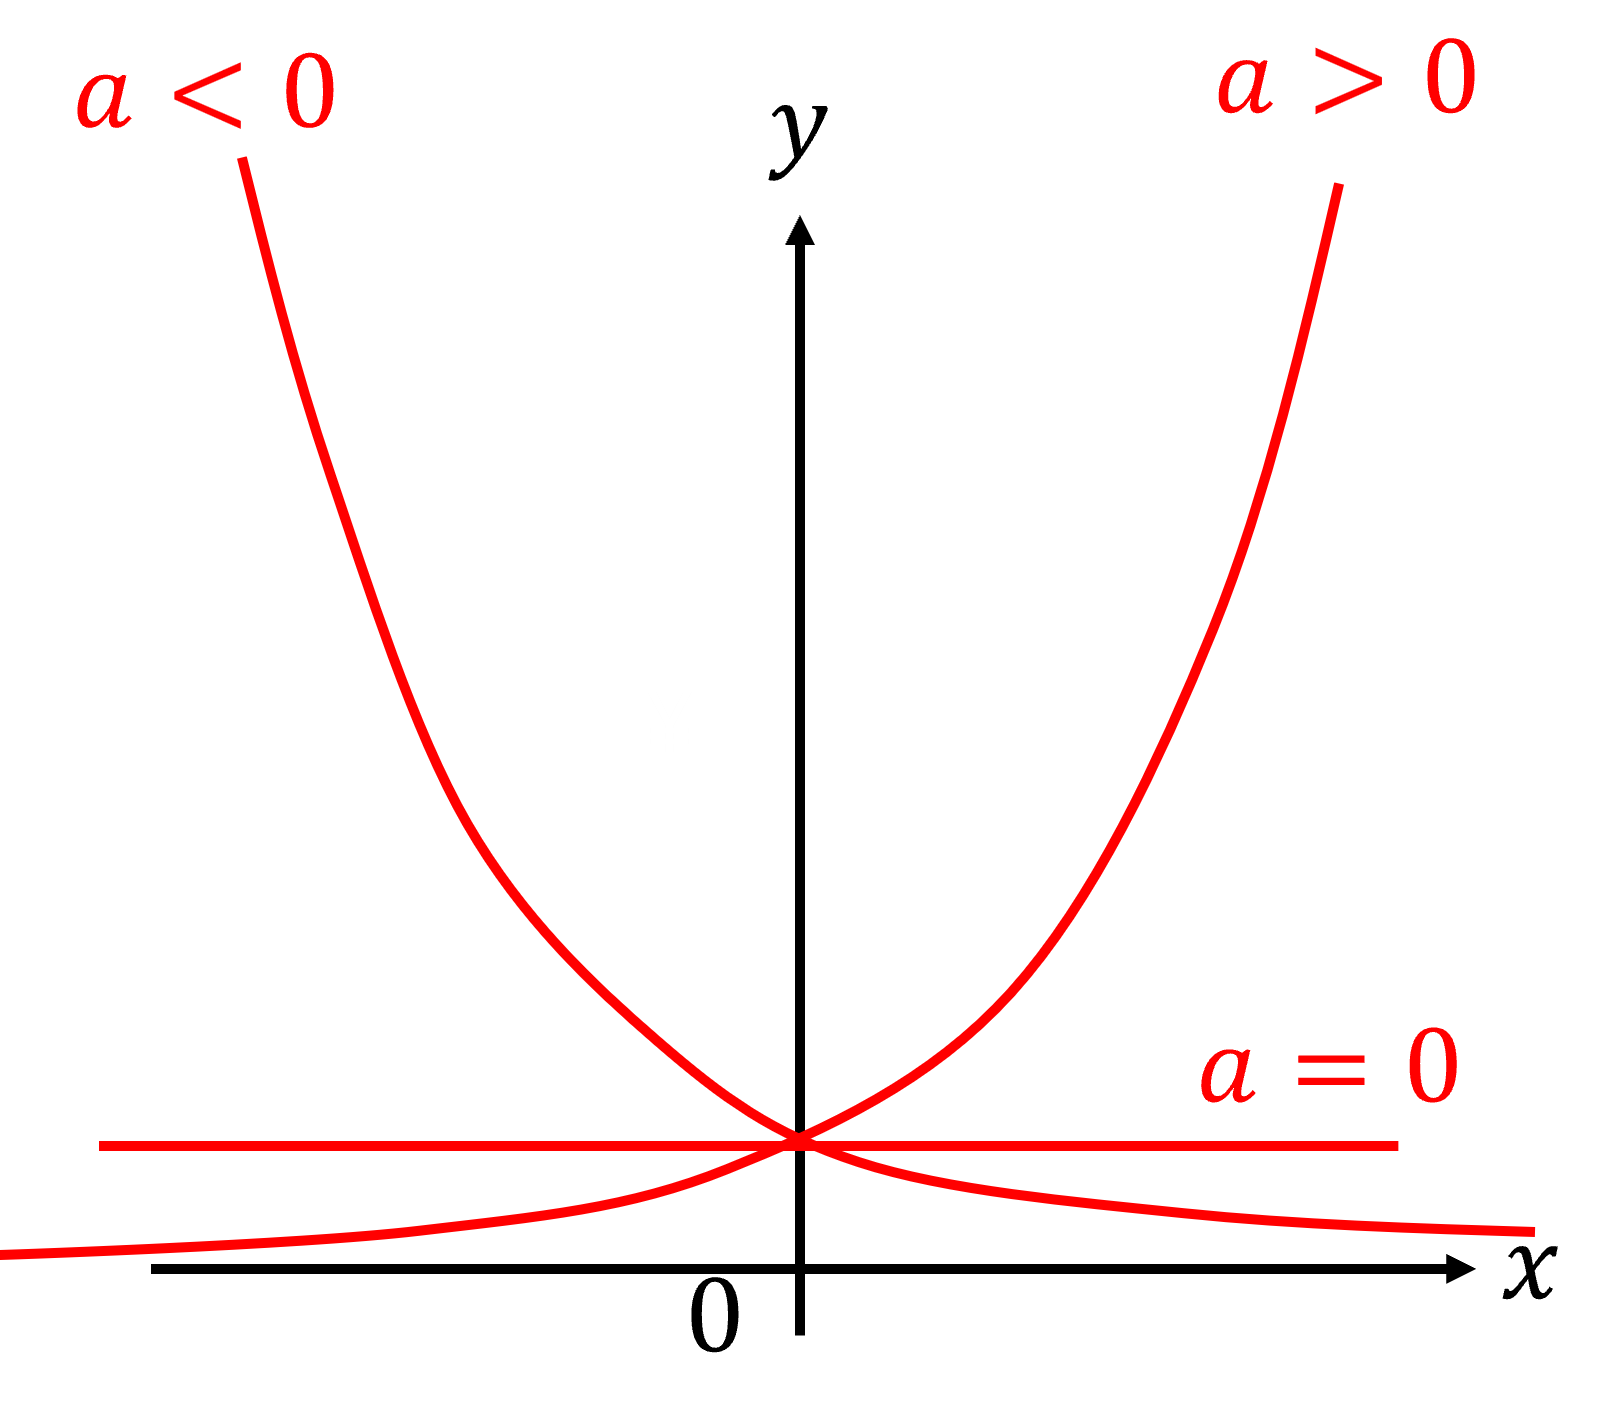
\includegraphics[width=50mm]{fig/1.png}
        \end{center}
    \end{figure}
\end{frame}
%---------------------------------------------------------------
\begin{frame}{指数と対数の基本関係}
    %! 指数と対数の基本関係, aダイナリ0, aノットイコール1, Mダイナリ0とする. 定義aのp乗イコールM, 同値pイコールログaのM, 特にログaのaイコール1, ログaの1イコール0, ログaのa分の1イコールマイナス1
    $a>0$, $a\neq 1$, $M>0$とする\par
    定義 $a^p=M \Leftrightarrow p=\log_a M $ \\
    特に $\log_a a=1, \log_a 1=0, \log_a \frac{1}{a}=-1$
\end{frame}
%---------------------------------------------------------------
\begin{frame}{対数の性質}
    %!対数の性質, abcは1でない正の数, Mダイナリ0, Nダイナリ0, kは実数とする. ログaのMNイコールログaのMプラスログaのN, ログaのN分のMイコールログaのMマイナスログaのN, ログaのMのk乗イコールkログaのM, ログaのbイコールログcのa分のログcのb, ログaのbイコールログbのa分の1
    $a$, $b$, $c$は1でない正の数\par
    $M>0$, $N>0$, $k$は実数とする
    \begin{eqnarray*}
        \log_a MN&=&\log_a M + \log_a N \\
        \log_a \frac{M}{N}&=&\log_a M - \log_a N \\
        \log_a M^k &=& k \log_aM \\
        \log_a b &=&\frac{\log_c b}{\log_c a} \\
        \log_a b &=& \frac{1}{\log_b a}
    \end{eqnarray*}
\end{frame}
%---------------------------------------------------------------
\begin{frame}{対数関数$y=\log_a x$とそのグラフ}
    %! 対数関数yイコールログaxとそのグラフ, yイコールログaのxはxイコールaのy乗と同値, 定義域はxダイナリ0, 値域は実数全体, aダイナリ1のとき, xが増加するとyも増加, 0ショウナリaショウナリ1のときxが増加するとyは減少, グラフは1_0を通り, y軸が漸近線
    \begin{itemize}
        \item $y=\log_a x$は$x=a^y$と同値 ($a>0$, $a\neq 1$)
        \item 定義域は$x>0$, 値域は実数全体
        \item $a>1$のとき $x$が増加すると$y$も増加
        \item $0<a<1$のとき $x$が増加すると$y$は減少
        \item グラフは点$(1_0)$を通り, $y$軸が漸近線
    \end{itemize}
    \begin{figure}[htbp]
        \begin{center}
            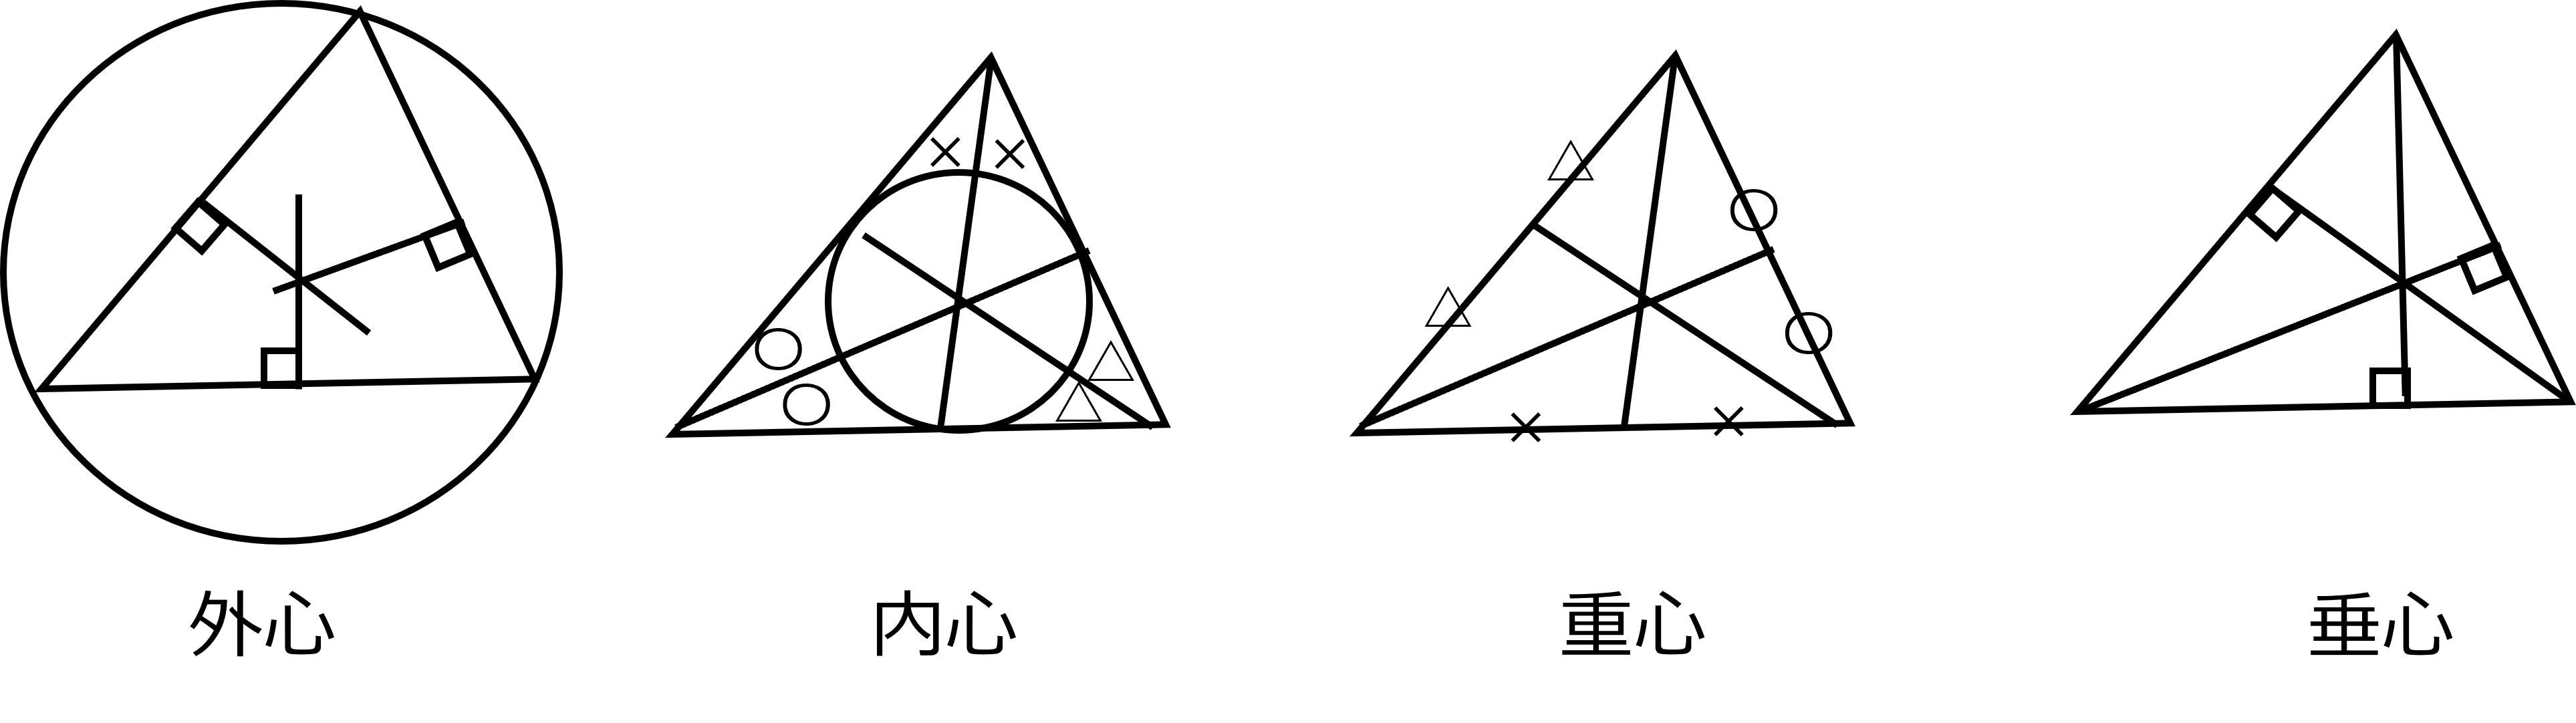
\includegraphics[width=50mm]{fig/2.png}
        \end{center}
    \end{figure}
\end{frame}



\end{document}
